\chapter{System Analysis}
System analysis is the performance management and documentation activities related to the life cycle phases of any software namely:
\begin{itemize}
	\item The Study Phase
	\item The Design Phase
	\item The Development Phase
	\item The implementation Phase
	\item The Testing Phase
\end{itemize}

In this stage, we gather information form the different sources for project development, we study about the existing system and its users, identifying system requirements, identifying actors, use cases and describing and illustrating them  using use case diagram, identifying business rules and describing sequence of message exchange, and sequence of activities,The methods of collecting information are : 
\begin{itemize}
	\item Interviewing
	\item Observations
	\item Viewing of documents and manuals from different sites
\end{itemize}

\section{Overview Of the Existing System}
The existing system of buying goods has several disadvantages. It requires lots of time to travel to the particular shop to buy the goods. It is having lots of manual work. Since everyone is leading busy life now a days, time means a lot to everyone. Also there are expenses for traveling from house to shop. It is less user-friendly. In current system user must go to shop and order products. It is difficult to identify the required product. More over the shop from where we would like to buy some thing may not be open all day and time. Hence we have to adjust our time with the shopkeeper's time or vendor's time. In current e-commerce system user have to go shop to view the description of the product. It is unable to generate different kinds of report.
   
The existing systems of e-commerce in Ethiopia sites lack many mandatory service that are expected from an e-commerce company plus there are very few companies that are organized(dedicated) only for e-commerce. For express we haven't seen express companies have online integrated delivery, ordering and live tracking mobile application. 

Lets take one local companies' that relates to our project's title deliveryaddis\footnote{Is and online food ordering and delivery companies, https://www.deliveryaddis.com/} how it works is you place your order through their website or mobile app any food you like and on the place order page you are asked to enter your location through either GPS or street name as-far it a good service but there are a couple of problems we found some of them listed below :-

\begin{itemize}
	\item Cost of delivery :- their coasting system is fixed with kilometers e.g 1-3 km 50 Birr ...
	\item Not realistic picture for the food
	\item No Live GPS tracking
\end{itemize}

The existing system of express companies (Delivery services) in Ethiopia is a manual one in which users are maintaing ledgers, books etc.. until recently to store the information like goods booking details, loading particulars, deliveries particulars, details of receivers of items at all branches, and customers details as well as employee details. It is very difficult to maintain historical data. Also regular investments need to purchase stationary every year.

General problems of existing systems found in Ethiopia are below.
\begin{itemize}
	\item Data may be lost or damage
	\item Any unauthorized person can access confidential data
	\item Any information cannot be easily searched
	\item Very little attention is given to forum 
	\item Products listed in some of the already made e-commerce sites are not what they say
	\item Companies that provide delivery service cost of delivery is not fixed it more of ranged by kilometers e.g 1-3 km 50 Birr 3-7 km 75 Birr and above 7km 100 Birr this kind of cost analysis  is not fair for customer with minim  kilometers
	\item Lack of websites' Lowest Denomination Design :-The websites made doesn't consider old phones but instead trays to keep up with new phone, from the perspective of the rapid change(developing) of technology is wonderful thing, but majority of Ethiopian peoples use old phone/browser even those technologies are outdated.
	\item Live GPS Parcel Tracking :- No body knows where their parcel is and how much time it take to reach the destined place (No Live Tracking).
	\item No Return Policy/Service :- Once you bought you bought it, their is no returning it weather the parcel is damaged or the item you expected, opened or have some cracking while delivering.
	\item No Customer Live Chat Support
	\item Drawback of the Inventory System
	\item Limited payment service :- cash on delivery
	\item It is difficult to maintain important delivery booking information in ledger
	\item More manual hour need to generate required reports form previous delivery history
	\item It is tedious to manage historical data which needs much space to keep all previous year's ledgers, books etc
	\item Daily transactions are to be entering into different books immediately to avoid conflicts which are very difficult
	\item No co-ordination between different branches because we are not storing the data at centralized location
\end{itemize}

\subsection{How existing system work}
Description of the event-flow present system is pointed out below:
\begin{enumerate}
	\item Client go to the nearest courier branch office and collect information about the destination branch office.
	\item The client calculate the cost for sending courier.
	\item Now client fill the form. The Details include in the form are
	\begin{itemize}
		\item Full name of sender
		\item Sender Mobile no 
		\item sender full address/Return address
		\item Mention the destination branch office 
		\item Mention this courier for home delivery or not.
		\item Full name of Receiver
		\item Receiver mobile no
		\item Receiver full address
	\end{itemize}
	\item Now Customer will hand over his or her good to the branch.
	\item If everything is okay way bill is printed out. it contains all the information to identify the delivery.
	\item  Then the data for a particular courier maintained in proper file.
\end{enumerate}

\subsection{Users Of The Existing System} 
\begin{itemize}
	\item Manufacturer
	\item Vendor
	\item Buyer
	\item Truck driver
	\item Mail sorters
\end{itemize}


\section{Overview Of The Developed System}
According to capitalethiopia\footnote{See https://www.capitalethiopia.com} website Ethiopia shows that annual growth for Internet users is at 37 percent and the number of active social media users is growing by 20 percent 
this growing use of Internet in Ethiopia provides a developing prospect for online shopping.

As we are well aware, most of our country people purchases products, exchange documents, buy foods, news papers by by going to store front, and it very tedious, tiring and takes lots of time finding the right product with an affordable(best) price range. In order to reduce this boring factors and make shopping, document exchange, food ordering, news paper ordering... fun, time saving and within our price range we introduce.

Guya E-commerce and Guya Express is an awesome application that empowers retailers large and small with their easy-to-use, easy-to-manage, customizable online store, secure checkout and live GPS tracking of their parcel. Guya E-commerce give you control over your look and  feel and allows any-one/any-seller to add products, manage your inventory, track sales, and more. As we go along building the project/application we'll focus on maximizing features to help improve customer experience. we'll include powerful search, product suggestion based on their product browsing history and categorization so customers can easily and quickly find what they're looking for. we use best practices so that product pages convert users to add more items to their shopping cart. And then most importantly, we guide people down the conversion funnel to complete the checkout process

Guya Express is vehicle based courier service in Ethiopia that specialize in safe delivery of any kind of parcels and their safe delivery in good condition and Guya E-commerce as the name suggests it is an online store for selling and buying products over the internet. Guya Express tracking system is web and mobile based system that helps customers to track the progress of their consignments online. It allows customers to visit the Guya Express's site or mobile application and enter their consignment number. The status of their consignment is displayed to the customer. The customer also have the provision to receive their consignment status by e-mail or SMS. The web-based online tracking system also allows branches to share information regarding the status of consignments among themselves. To summarize, the online courier tracking system offers the following advantages:
\begin{itemize}
	\item It offers real-time Parcel statuses to its customers
	\item It decreases wrongly routed consignment
	\item Information sharing between branches which allows the  client to improve their operation 
\end{itemize}

%In our project, we propose the development of e-commerce with express

The design an layout of the application will be Search Engine Optimization(SEO) friendly constructed using css XHTML, DHTML alogn with use of AJAX and non-blocking I/O this is because of makeing the user wait for all thing be made in server an sending it  all together why not load the web page static files like logos, buttons... send the database query when it is done this way we'll rich user interface experience i.e asynchronous static file retrieval and keeping in mind the latest web trends.

There basically two way of selling on Guya E-commerce Guy Vendor Central and Guya Seller Central

\paragraph{Guya Vendor Central}
Vendor Central is an invite-only program. Guya Vendor Central grants Guya ownership of your inventory, which will market and sell to shoppers on the website.

How It Works : Merchants or manufactures sell their inventory (e.g hats) on Guya at wholesale rates. Once those items have been sent to Guya, the seller is done with the products. Guya pays for the inventory directly to the seller and maintains ownership of the products. Guya sells those products on the Marketplace (as Guya) i.e choosing their own price and shipping options.

\subparagraph{Benefits of using Guya Vendor Central}
Selling to Guya is an available option for manufactures and virtually eliminates direct seller work including marketing, advertising, and even pricing.

Other benefits of Selling to Guya include:

\begin{itemize}
	\item Avoid the hassle of handling pricing, shipping and other logistics for product sales
	\item Bulk purchases
	\item Display and detail page functionality only available to Guya (e.g subscribe and save)
	\item Manufacturer Central inventory projection tools not available in Seller Central
\end{itemize}

\paragraph{Guya Seller Central}
Unlike Guya Vendor Central, sellers on Guya Seller Central maintain ownership of their inventory and sell under their own brand name.

How It Works: Sellers list their products on the Guya Marketplace, and sell items as 3rd party sellers.

Selling through Guya Seller Central is generally more work than selling through Guya Vendor Central, but it also comes with greater levels of control and the potential for higher margins. Sellers on the Marketplace control shipping, price and optionally fulfillment. Sellers who sell on the Guya Marketplace have different fulfillment options to choose from. Sellers can choose whether they want to handle fulfillment or let Guya sort, package and ship products through their own fulfillment centers.

As a third party seller selling on the Guya Marketplace you have the option to use Guya's fulfillment services:

\begin{itemize}
	\item Fulfilment by Guya (FBG) - Sellers leverage Guya's fulfilment for products sold on the Guya Marketplace
	\item Sell Using your own fulfillment (FBV) - Sellers handle fulfillment for their products sold on the Guya Marketplace
\end{itemize}

\paragraph{Benfits of using Guya Marketplace}
\begin{itemize}
	\item Increase Exposure - Leverage millions of unique monthly visitors to get more people to your online store.
	\item Leverage Marketplace Benefits - Guya's Marketplace is a hopping destination that is known for reliability, ease of online shopping and selection. Listing on the Marketplace allows sellers to capitalize on that branding 
	\item Find New Customers - The Guya Marketplace is huge. Sellers gain exposure to new and varied shoppers through the Marketplace - man of which would never encounter your online store otherwise.
	\item Increase Sales - Shoppers on Guya have come to the Marketplace with the explicit intent to purchase, or at the very least are looking to browse. Online search, advertising and other forms of online exposure do not guarantee that same bottom of the funnel-audience. Bottom Line - people on Guya are more likely to buy.
\end{itemize}


Here is an overview of the features for each way we can sell on Guya:

\begin{table}%[H]
\begin{tabular}{|p{3cm}|p{3cm}|p{3cm}|p{3cm}|}
\hline
Name & Sell to Guya & Sell on Guya (FBG) & Sell on Guya (FBV) \\
\hline
Product Placement & Guya Marketplace & Guya Marketplace & Guya Marketplace \\
\hline
Product Seller & Guya & Seller & Seller \\ 
\hline 
Product Price Controlled by & Guya & Seller & Seller \\
\hline
Product Shipping handled by & Guya & Guya & Seller \\
\hline
Product Returns Handled by & Guya & Guya & Seller \\
\hline
\end{tabular}

\caption{Overview of selling on Guya E-commerce}
\label{selling_on_guya_table}

\end{table}

\paragraph{Advantages of Proposed System:}
The following are the advantages of proposed systems
\begin{description}
	\item[Convenience : ] This is one of the main reasons that online shopping has become so popular, as it allows you to switch stores and products by clicking a button rather than traveling to a new store.
	\item[Selection : ] Of course, a large selection means that your decision making process may be a bit more difficult, but is also makes it more likely that you will find a high quality product that truly pleases you.
	\item[Immediacy : ] When you purchase a new product, whether for yourself or for another person, it is always nice to have that product in your possession immediately.
	\item[Quality : ] Needless to say, the quality of a product is also very important. And, while most online shopping offers you the ability to return faculty or imperfect product.
	\item[Saving Money : ] Another very important aspect of any shopping experience is trying to save as much money as possible. One reason that people enjoy online shopping is that you can often find a product more cheaply online that you can in stores.
	\item[Discounts and offers : ] Yes online shopping is better than offline because we can shop at any of our favorite shop and can get the delivery on same day itself.
	\item[Less time consuming : ] Work carried out by the staff at various stages will be less time consuming.
	\item[Safety : ] The system will be accessible by only the authorized users. As information, being the most crucial for the organization, then the safety of information is important.
	\item[Routing Information : ] A Sender can see the all routing information and estimated date of delivery.
	\item[Be update : ] Client get all update via Email or SMS about courier e.., whether packet is delivered, pending or returned the courier.
	\item[Online chat room : ] User can chat with company through online chat room.
	\item[Online tracking system : ] A customer can track the parcel and identify the location.
\end{description}
%\begin{itemize}
%	\item Easy to manage all the daily transactions
%	\item Centralized database help in avoiding confilicts between different branches
%	\item Avoid/Reduce human errors
%	\item Provide better customer support from any branch
%	\item Can generate required reports easily
%	\item Easy to manage historical data in a secure manner
%	\item Easy to use UI that does not requires specific training
%\end{itemize}


%\section{Overview Of The Microservices}
%\subsection{User Service}
%\subsection{Order Service}
%\subsection{Catalog Service}
%\subsection{Inventory Service}
%\subsection{Gatekeeper Service}
%\subsection{Payment Service}
%\subsection{Pricing Service}
%\subsection{Logging Service}
%\subsection{Xpress Service}
%\subsection{Storybook Repository}
%\subsection{Bits Repository}
%\subsection{Guya's Cascading Style Sheets (GCSS)}
%\subsection{Python Logstash}
%\subsection{Alfa-Geez Node Repository}
%\subsection{Tracking Service}
Tracking is the technology used to determine the location of a vehicle using different methods like GPS and
other navigation system operating via satellite and ground based stations.

% Diagram of tracking(Block diagram)
%\subsubsection{Active and passive tracking}


\section{System Requirement Specification}
General structure of a user story described in this document: 
\\ \\
\begin{normalsize}
\textbf{\{User story name\}}: As a \{role\}, I want \{goal\}, so that \{benefit\} (\{priority\}).
\end{normalsize}

\subsection{Functional Requirements}
\subsubsection{Browse Products}

\begin{description}
	\item[List products:] As a customer, I want to list all products of the shop (1).
	\item[Filter by category:] As a customer, I want to see only those products that belong to a particular category and any category descendant, so that I can narrow down the list to what fits best my needs (2).
	\item[Filter by price:] As a customer, I want to see only those products from the product list which prices fall within a specific price range, so that I can narrow down the list to best fit my economic requirements (3).
	\item[Filter by color:] As a customer, I want to see only those products from the product list which main color matches any of the colors I selected, so that I can narrow down the list to best fit my liking (4).
	\item[Sort by name:] As a customer, I want to sort the products from the product list by their name in an ascendant or descendant order (9).
	\item[Sort by price:] As a customer, I want to sort the products from the product list by their price in an ascendant or descendant order (8).
	\item[Pagination:] The product list needs to be displayed divided into pages and the customer should be given the ability to browse through them (3).
	\item[Product detail:] As a customer, I want to see all information regarding a particular product and its variants, so that I can make a better decision about buying it (1).
	\item[Breadcrumb:] As a customer, I want to be informed of my location inside the category tree via a breadcrumb, so that it can help me to navigate and have a better understanding of the web-shop structure (6).
	\item[Empty list message:] As a customer, I want to be informed with an informative message when a product list request has no results (5).
	\item[Not found message:] As a customer, I want to be informed with an informative message
when a category or product I requested cannot be found (10).
\end{description}

\subsubsection{Purchase Products}
\begin{description}
	\item[Add item to cart:] As a customer, I want to add a particular product to the shopping cart, so that I can buy it with the next order (1).
	\item[Update item in cart:] As a customer, I want to change the number of units of a particular item in the shopping cart, so that I can buy a different quantity of the product with the next order (6).
	\item[Remove item from cart:] As a customer, I want to remove a particular item from the shopping cart, so that I do not buy it with the next order (3).
	\item[Place order:] As a customer, I want to place an order, so that I can actually buy the items in my shopping cart (2). 
	\item[Payment:] As a customer, I want to be able to pay online my orders, so that I can pay immediately the moment I buy them instead of using other possibly unpleasant billing options (4). 
	\item[List orders:] As a registered customer, I want to see a list of my orders, so that I can see all the purchases I did in the past (5). 
	\item[Mini cart:] As a customer, I want to be able to see my current shopping cart from any page via a so-called mini-cart, so that I can always be aware of its contents and pricing details (5).  
\end{description}	
  
\subsubsection{User Management}
\begin{description}
	\item[Sign up:] As an anonymous customer, I want to sign up a new customer account, so that I can place orders more easily and take advantage of many other benefits (4).
	\item[Log in:] As an anonymous customer, I want to log in with an existing customer account, so that I take advantage of the benefits of being a registered customer (4).
	\item[Log out:] As a registered customer, I want to logout from my customer account, so that nobody else can use it from the same machine (5).
	\item[Recover password:] As an anonymous customer, I want to be able to recover my password, so that I can log in with my account when I forget my current password (7).
	\item[Update account:] As a registered customer, I want to update my personal data such as the email address used (6).
	\item[Change password:] As a registered customer, I want to change my current password to another one of my choice (5).
	\item[Add address:] As a registered customer, I want to add a postal address to my address book, so that I can select it as shipping or billing address when placing an order (5).
	\item[Update address:] As a registered customer, I want to update the data of a particular postal address from my address book, so that it corresponds to my current situation (6).
	\item[Remove address:] As a registered customer, I want to remove a particular postal address from my address book, so that I cannot longer select it when placing an order (5).
\end{description}

\subsection{Non-functional Requirements} 
The non-functional requirements involved to perform the implementation of e-commerce and express database and source code are as listed below.

\paragraph{Normalization}
The basic objective of normalization is to reduce redundancy which means that information is to be stored only once. Storing information several times leads to wastage of storage space and increase in the total size of the data stored.

If a database is not properly designed it can give rise to modification anomalies. Modification anomalies arise when data is added to, changed or deleted from a database table. Similarly, in traditional databases as well as improperly designed relational databases, data redundancy can be a problem. These can be eliminated by normalizing a database.
 
Normalization is the process of breaking down a table into smaller tables. So that each table deals with a single theme. There are three different kinds of modifications of anomalies and formulated the first, second and third normal forms (3NF) is considered sufficient for most practical purposes. It should be considered only after a thorough analysis and complete understanding of its implications.

\paragraph{Safety}
It there is extensive damage to a wide portion of the database due to catastrophic failure, such as disk crash, the recovery method restores a past copy of the database that was backed up to archival storage (typically tape) and reconstructs a more current state by reapplying or redoing the operations of committed transactions from the backed up log, up to the time of failure.

\paragraph{Performance Requirements}
\begin{itemize}
	\item The product shall be based on web and has to be run form a web server or Cloud.
	\item The product shall take initial load time depending on internet connection strength which also depends on the media from which the product is run.
	\item  The performance shall depend upon hardware components of the client/customer.
\end{itemize}

\paragraph{Security}
Security system need database storage just like many other applications. However, the special requirements of the security market mean that vendors must choose their database partner carefully.
\begin{itemize}
	\item The database system has to be secure to prevent unauthorized access, theft and/or disruption to data and services held and offered by the system.
	\item The system's back-end servers shall only be accessible to authenticated administrators.
	\item The system's back-end databases shall be encrypted.
\end{itemize}

\paragraph{Scalability}
\begin{itemize}
	\item The system will begin offering its service to a small number of users but must be capable of being upgraded to serve larger number of users and process more transactions.
\end{itemize}

\paragraph{Robustness}
\begin{itemize}
	\item The system should be able to operate and handle various types of data needed to function properly.
\end{itemize}

%\paragraph{Efficiency}
%\begin{itemize}
%	\item 
%\end{itemize}

%\paragraph{Maintainability}
%\begin{itemize}
%	\item Repair time shall be within an hour.
%\end{itemize}

\paragraph{Availability}
The web-site should be available on the specified date and specified time as many customers are doing advance buying selling delivery.

%\paragraph{Correctness}

%\paragraph{Usability}

\paragraph{Supportability}
\begin{itemize}
	\item There are no memory requirements in client's side.
	\item The computers must be equipped with any of the web browsers.
	\item The product must be stored in such a way that allows the client easy access to it.
	\item Response time for loading the product should take no longer than five minutes.
	\item A general knowledge of basic computer skills is required to use the product.
\end{itemize}

%\subsubsection{Technical Requirements}

\subsection{Business Rules}
\begin{description}
	\item[BR1:] For using systems functionality customers are required to sign-up.
	\item[BR2:] Consumer customers are not required any subscription fee.
	\item[BR3:] Merchants are required subscription fee.
	\item[BR4:] Any Customers are subjected to taxation.
	\item[BR5:] Monthly subscribed vendors are the only ones that can use fulfillment by Vendor method. 
	 subscription fee.
\end{description}


\section{System Requirement Analysis}
\subsection{Actor and Use Case Identification}
A use case diagram is a graphic depiction of the interactions among the elements of a system. A use case is a methodology used in the system analysis to identify, clarify, and organize system requirements in this context, the term \"system" refers to something being developed or operated such as a mail-order product sales and service website. Use case diagram are employed in UML (Unified Modeling Language). A standard notation for the modeling of real-world object and systems. System objectives can include planning overall requirements validating a hardware design, testing and debugging a software product under development, creating an online help reference, or performing a consumer-service oriented task. For example, use case in a product sales environment would include item ordering, catalog updating payment processing, and customer relations. A use case diagram contains four components.
\begin{itemize}
	\item The system boundary, which defines the system scope or boundary in accordance to
the real world around it.
	\item Use case actors are individuals or users involved in the system. Each actor has
different roles or actions to perform in the system.
	\item The use cases specify the scenarios or possible outcome that can be performed by
the actors in the system.
	\item The relationships between the actors and the use cases represents the possible
scenarios and outcomes, it shows how system behaves according to different scenario
and actor.
\end{itemize}

Below is a list of the elements that you will see in the diagram on the next page as well what is included in the use case templates that follow. 

\begin{tabular}{|p{2cm}|p{3cm}|p{9cm}|}
\hline 
\rule[-1ex]{0pt}{2.5ex} \textbf{Name} & \textbf{Diagram} & \textbf{Description} \\ 
\hline
\rule[-1ex]{0pt}{2.5ex}Actors & • & Shown in the diagram as stick figures with a name underneath. They represent elements that will be directly interacting with the system. \\ 
\hline 
\rule[-1ex]{0pt}{2.5ex}Use Cases & • & Oval shapes that have their names in the center. These represent direct functionality within the system that must be implemented. \\ 
\hline 
\rule[-1ex]{0pt}{2.5ex}Interactions & • & Lines that connect the actors with the different Use Cases. These show that there is some form of direct interaction between the actor and that specific functionality. \\ 
\hline 
\rule[-1ex]{0pt}{2.5ex}Includes & • & Dotted lines labeled "$<<$include$>>$" that connect two use cases and have an arrow pointing towards one. This means that the use case without the arrow calls on the functionality of the use case with the arrow. \\ 
\hline 
\rule[-1ex]{0pt}{2.5ex}Extends & • & Dotted lines labeled "$<<$extend$>>$" that connect two use cases and have an arrow pointing towards one. This means that the use case without the arrow takes all of the functionality of the use case with the arrow and adds extra functionality. \\ 
\hline 
\rule[-1ex]{0pt}{2.5ex}The System Boundary & • & The large rectangle that contains the Use Cases. Everything within the rectangle is what the system is responsible for implementing. \\ 
\hline 
\rule[-1ex]{0pt}{2.5ex}Use Case Template & • & Describes the basic functionality and features of each use case and the can be found in the pages following the use case diagram. \\ 
\hline 
\end{tabular} 




\subsubsection{Actor identification}
\paragraph{E-commerce Actor identification}
The top level actors that interact with the system are the customer, the Website Administrator, the identity manager, the warehouse manager, the warehouse clerk, the customer service and the marketing administrator. The customer can be an anonymous customer or an identified customer. The identified customer can be a vendor, a consumer or both for a better understanding the generalization of actors are illustrated in figure \ref{shop_actors}.
\begin{figure}[!h]
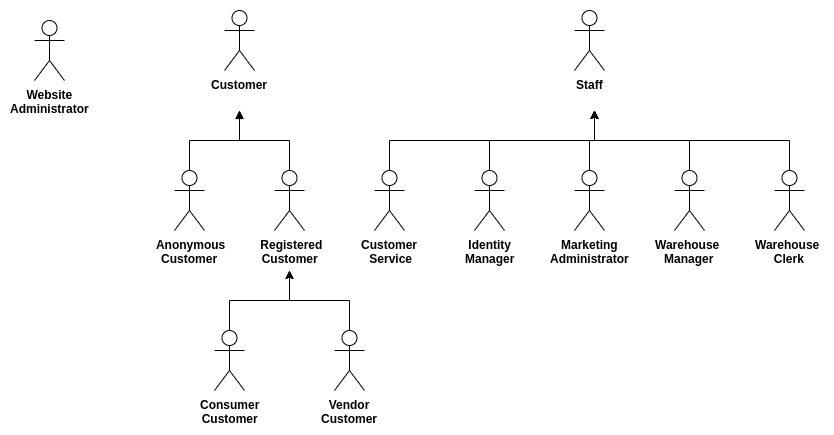
\includegraphics[width=13cm, keepaspectratio]{images/shop_actors}
\label{shop_actors}
\caption{Actors involved - Guya E-commerce}
\end{figure}

\begin{description}
	\item[Website Administrator:] The Admin works with the different facility that help to solve the problem of manual work and contact can be easily maintain with the all branches. It's job includes the following:
	\begin{itemize}
		\item Set default language
		\item Set taxation rate
		\item Set Term and Conditions
		\item Set Privacy Policies
		\item Managing user groups and setting different privileges
		\item Managing user sessions
		\item Logs
		\item Staff allocation
		\item Staff revocation
		\item Branch creation
		\item Branch termination	
	\end{itemize}
	\item[Identity Manager:] Is used to ensure that users (customers) provide information that is associated with the identity of a real person. This management service verity the authenticity of physical identity documents such as:
	\begin{itemize}
		\item Drivers license
		\item Passport
		\item Residential proof
	\end{itemize}
	\item[Customer Service:] Is majorly concerned with customer relation including:
	\begin{itemize}
		\item Check delivery status
		\item Take customer's feedback
		\item Mange customers to some extent 
	\end{itemize}
	\item[Marketing Administrator:] Refers to activities undertaken to promote the buying and selling of products or services.
	\begin{itemize}
		\item Make Link click through sales commission
		\item Make physical (delivery) item promotion (e.g. sample soaps, perfumes...)
		\item Set a discount price or rate
		\item Label items (e.g. Assured quality)
		\item Set price to catalogs
		\item Add new department
		\item Remove department
		\item Send promotion Email, SMS
		\item Create promotion i.e. deal of the day 
		\item Make featured product
		\item Create discount/fee coupon for items
		\item Forecast inventory in warehouse (can be done automatic or manually)
		%\item Update stocks
		%\item add/remove stocks
	\end{itemize}
	\item[Warehouse Manager:] It is related to quantitative value of products, the quantitative value of products is managed by tow way one is automatic update that is done when a product is ordered or returned, the other is done while stocking the warehouse or removing stocks (that is done manually by the warehouse manager     
	\item[Warehouse Clerk:] Fulfillment of orders  	
	\begin{itemize}
		\item Viewing Orders in order to pack
		\item Responsible with returned orders
	\end{itemize}
	\item[Anonymous Customer:] (Is generalized under actor name Customer) Is an registered person who comes to the website to sell, buy or browse catalogs. visitors are allowed to:
	\begin{itemize}
		\item View catalogs
		\item View available departments
		\item Add catalogs to cart
		\item View available stores
		\item checkout (but in checkout they are required to register)
		\item Signing up
		\item Report illegal sales i.e. copyright, adultery contents
	\end{itemize}
	\item[Vendor:] (Is generalized under actor name Customer) Is a person or a company offering inventory/stocks for sale. Vendors functionality include the following:
	\begin{itemize}
		\item Add catalogs
		\item Remove catalogs
		\item Set pricing to catalogs
		\item Make a discount
		\item Send/Make promotion based on Consumer's choice
		\item Add multiple self fulfillment centers address
		\item Set return policy for catalogs based on fulfillment plan
	\end{itemize}
	\item[Consumer] (Is generalized under actor name Customer) Is an individual who pays some pays some amount of money for catalog to consume goods and services.
	\begin{itemize}
		\item View store
		\item Rate a store
		\item Order items
		\item checkout
		\item Add catalog to wish list
		\item Subscribe for physical item promotion (e.g. sample soaps, perfumes...)
		\item Register for link click through sales commission
		\item Report illegal sales i.e. copyright, adultery contents
	\end{itemize}
\end{description} 

\paragraph{Express Actor identification}
The top level actors that interact with the system are listed below and the generalization of actors are illustrated in figure\ref{express_actors}.
\begin{description}
	\item[Customer:] Customers can use various service by online with the help of internet. These services help the user to do their work effectively and efficiently. The services are following:-
	\begin{itemize}
		\item Pickup Request
		\item Destination Locator
		\item Track Locator
		\item Rate Calculator
		\item Consignment Guidelines
	\end{itemize}
	\item[Website Administrator:] The Website Administrator works with the different facility that help to solve the problem of manual work and contact can be easily maintain with the all branches. It's job includes the following:-
	\begin{itemize}
		\item Branch creation
		\item Branch termination
		\item Send message
		%\item User request 
		%\item Request 
		\item Staff allocation
		\item Staff revocation
		\item View report
	\end{itemize}
	\item[Delivery Guy:] (Is generalized under actor name Staff) Is the person who delivers parcels to customers usually over a regular local route some of responsibility includes :-
	\begin{itemize}
		\item Collect payments from customer at the time of product delivery
		\item Take customer signature for proof of delivery (POD) at the time of product delivery
		\item Pick up parcels-
	\end{itemize}
	\item[Front Desk Receptionist:] (Is generalized under actor name Staff) Responsible for handling front office reception, also serves as a Customer Support/Service some of the services include :-
	\begin{itemize}
		\item Receive parcels and collect payment for those
		\item Check for delivery status (tracking of parcels)
		\item Provide enter form for customers and printing labels for those parcels
	\end{itemize}
\end{description} 

\begin{figure}[!h]
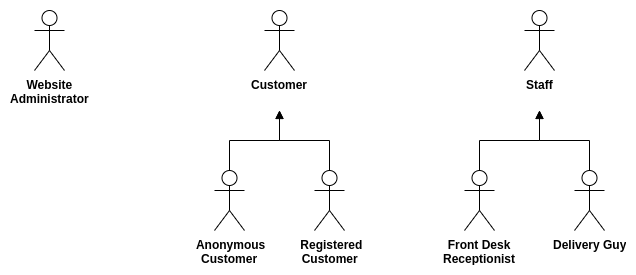
\includegraphics[width=13cm, keepaspectratio]{images/express_actors}
\label{express_actors}
\caption{Actors involved - Guya Express}
\end{figure}


\subsubsection{Use Case Diagram And Description}
Website security requirements mandate separation of administrative interface from common functions provided to users. This segregation, for example, is strongly recommended by ISO 17799.

System should have separate application for administrators and for common users. It is recommended by OWASP Guide 2.0\footcite{https://www.owasp.org} that website administration application should not be accessible from  the internet without going through some management networks eg. via a strongly authenticated VPN or from a trusted network operation center.

Except for administrators, some part of the administrative interfaces should be also available to the Help desk staff (Customer Service) and some staffs, as they need to be able to assist customers having issues while using the customer oriented website.

Top level use case diagram below shows some administrative functions that administration website could provide.

\paragraph{Administrative Use Case Diagram}
\begin{figure}[!hb]
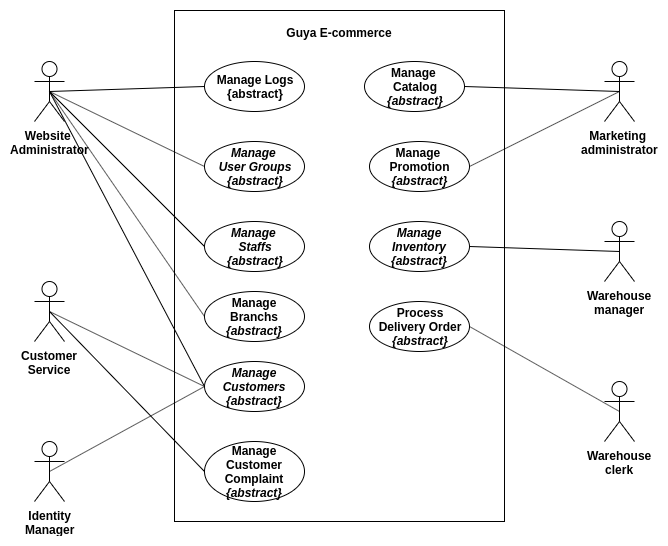
\includegraphics[width=15cm,keepaspectratio]{usecases/shop_admin_top_level_usecase}
\caption{Top level use case diagram for the administration website - Guya E-commerce}
\end{figure}

\subparagraph{Manage Logs}
Website administrator see status of logs. The status could include verification that logging is stil functional (there is enough space on disk and/or connection to database is not stable), and that older log files are on schedule being moved to a permanent storage for archiving. List of administrative functions include in the log management depend on the security requirements supported and implemented by the website, which we will detail on the implementation phase.

Logs accessing is not associated with our system, but we will be implementing logging functionality that is stored as a text file not in database, instead the website administrator view logs using either the file manager form web hosting provided panel or FTP.

%################################# Manage Logs #############################
\begin{figure}[!ht]
\centering
%\vspace*{-8cm}
%\hspace*{-3cm}
%\noindent
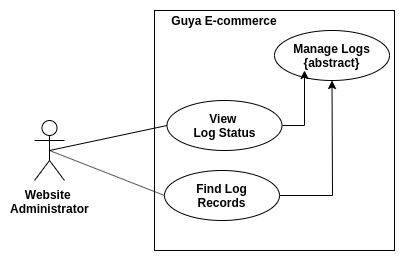
\includegraphics[width=10cm,keepaspectratio]{usecases/manage_logs_usecase_admin}
\caption{Manage logs use case diagram for administration website - Guya E-commerce}
\end{figure}
%################################# End Of Manage Logs ############################# 

%################################# Manage user groups #############################
\begin{figure}[!ht]
\centering
%\vspace*{-8cm}
%\hspace*{-3cm}
%\noindent
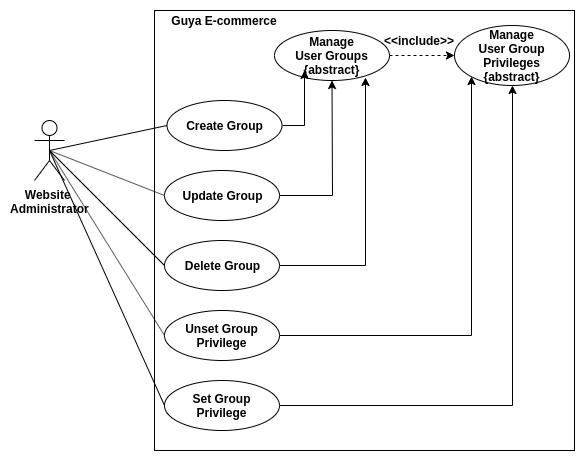
\includegraphics[width=10cm,keepaspectratio]{usecases/manage_user_groups_usecase}
\caption{Manage user groups use case diagram for administration website - Guya E-commerce}
\end{figure}
\begin{table}[!h]
\begin{tabular}{|l|p{6cm}|p{6cm}|}
\hline 
\rule[-1ex]{0pt}{2.5ex} \textbf{Use Case Name} & \multicolumn{2}{p{10cm}|}{Manage User Groups} \\ 
\hline 
\rule[-1ex]{0pt}{2.5ex} \textbf{Description} &\multicolumn{2}{p{10cm}|}{The idea is that website administrator could create different user groups, for example having different privileges or options, and later some user groups could be modified or even deleted} \\ 
\hline 
\rule[-1ex]{0pt}{2.5ex} \textbf{Primary Actor}& \multicolumn{2}{p{10cm}|}{Website Administrator} \\ 
\hline 
\rule[-1ex]{0pt}{2.5ex} \textbf{Pre-Condition} & \multicolumn{2}{c|}{User has been logged on to system} \\ 
\hline 
\rule[-1ex]{0pt}{2.5ex} \textbf{Post-Condition} & \multicolumn{2}{p{10cm}|}{}  \\ 
\hline 
\multirow{4}{*}{\textbf{Basic Flow}} & \textbf{Actor Action} & \textbf{System Response}\\
\cline{2-3}
%
&
\textbf{1.}  The Use Case starts when the user is logged on to the website and select the manage user groups menu.
& 
\textbf{2.}  The system will display lists of user groups.
\\
%
&
\textbf{3.}  The user will select create new user group.
& 
\textbf{4.}  The system will display form for creating new user group with group name, group id, list of privileges. 
\\
%
&
\textbf{5.}  The user will fill the displayed from and submit the form.
& 
\textbf{6.}  The system will verify the information like if the data is redundant or not and store the user group information. 
\\
%
&

& 
\textbf{7.}  The Use Case ends. 
\\
\hline 
\rule[-1ex]{0pt}{2.5ex} \textbf{Alternate Flow} & \multicolumn{2}{p{10cm}|}{\textbf{A1 : } If the website administrator requests to edit an existing user group then:}  \\ 
\cline{2-3}
\multirow{2}{*}{} & \textbf{Actor Action} & \textbf{System Response}\\
\cline{2-3}
%
&
\textbf{2.1}  The user click edit button/icon for the listed user groups. 
& 
\textbf{2.2}  The system display the same form as creating new user group, but filled with the selected user group information. 
\\
%
&
\textbf{2.3}  The user edits the options and submit the form. 
& 
\textbf{2.4}  The flow continues to Basic flow 6  
\\
\cline{2-3}
\rule[-1ex]{0pt}{2.5ex} & \multicolumn{2}{p{10cm}|}{\textbf{A2 : } If the website administrator requests to remove an existing user group then:}  \\ 
\cline{2-3}
\multirow{2}{*}{} & \textbf{Actor Action} & \textbf{System Response}\\
\cline{2-3}
%
&
\textbf{2.1}  The user click remove button/icon for the listed user groups. 
& 
\textbf{2.2}  The system display confirmation message. 
\\
%
&
\textbf{2.3}  The user confirms. 
& 
\textbf{2.4}  The system will set all the users under the removed user group to default user group i.e no user group and remove the user group safely.
\\
\hline
\end{tabular}
\caption{Manage logs use case description - Guya E-commerce} 
\end{table}

%################################# End Of Manage user groups #############################

%################################# Manage staffs #############################
\begin{figure}[!ht]
\centering
%\vspace*{-8cm}
%\hspace*{-3cm}
%\noindent
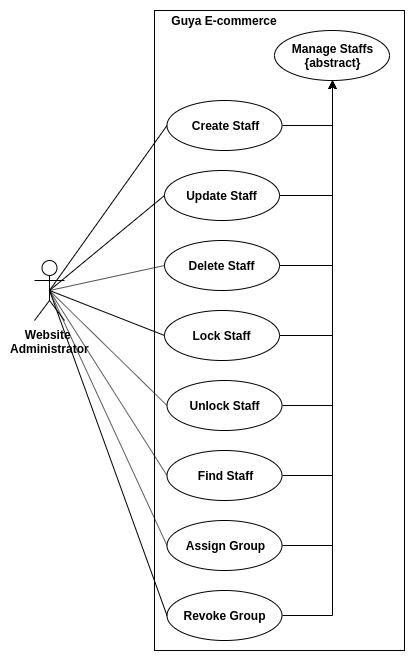
\includegraphics[width=10cm,keepaspectratio]{usecases/manage_staffs}
\caption{Manage staffs use case diagram for administration website - Guya E-commerce}
\end{figure}
\begin{table}[!h]
\begin{tabular}{|l|p{6cm}|p{6cm}|}
\hline 
\rule[-1ex]{0pt}{2.5ex} \textbf{Use Case Name} & \multicolumn{2}{p{10cm}|}{Manage Staffs} \\ 
\hline 
\rule[-1ex]{0pt}{2.5ex} \textbf{Description} &\multicolumn{2}{p{10cm}|}{Is the management of subordinates in the organization, manage staffs refers to the administrative actors} \\ 
\hline 
\rule[-1ex]{0pt}{2.5ex} \textbf{Primary Actor}& \multicolumn{2}{p{10cm}|}{Website Administrator} \\ 
\hline 
\rule[-1ex]{0pt}{2.5ex} \textbf{Pre-Condition} & \multicolumn{2}{c|}{User has been logged on to system} \\ 
\hline 
\rule[-1ex]{0pt}{2.5ex} \textbf{Post-Condition} & \multicolumn{2}{p{10cm}|}{}  \\ 
\hline 
\multirow{4}{*}{\textbf{Basic Flow}} & \textbf{Actor Action} & \textbf{System Response}\\
\cline{2-3}
%
&
\textbf{1.}  The Use Case starts when the user is logged on to the website and select the manage staffs menu.
& 
\textbf{2.}  The system will display lists of staffs.
\\
%
&
\textbf{3.}  The user will select create new staff.
& 
\textbf{4.}  The system will display form for creating new staff with staffs personal info, username, password, branch and user group. 
\\
%
&
\textbf{5.}  The user will fill the displayed from and submit the form.
& 
\textbf{6.}  The system will verify the information like if the data is redundant or not and store the information. 
\\
%
&

& 
\textbf{7.}  The Use Case ends. 
\\
\hline 
\rule[-1ex]{0pt}{2.5ex} \textbf{Alternate Flow} & \multicolumn{2}{p{10cm}|} { \textbf{A1 : } If the website administrator requests to edit an existing staff then:}  \\ 
\cline{2-3}
\multirow{2}{*}{} & \textbf{Actor Action} & \textbf{System Response}\\
\cline{2-3}
%
&
\textbf{2.1}  The user click edit button/icon for the listed staff. 
& 
\textbf{2.2}  The system display the same form as creating new staff, but filled with the selected staff's information. 
\\
%
&
\textbf{2.3}  The user edits the options and submit the form. 
& 
\textbf{2.4}  The flow continues to Basic flow 6  
\\
\cline{2-3}
\rule[-1ex]{0pt}{2.5ex} & \multicolumn{2}{p{10cm}|} { \textbf{A2 : } If the website administrator requests to remove an existing staff then:}  \\ 
\cline{2-3}
\multirow{2}{*}{} & \textbf{Actor Action} & \textbf{System Response}\\
\cline{2-3}
%
&
\textbf{2.1}  The user click remove button/icon for the listed staff. 
& 
\textbf{2.2}  The system display confirmation message. 
\\
%
&
\textbf{2.3}  The user confirms. 
& 
\textbf{2.4}  The system delete assigned branch, login info, delete assigned user group but personal info is preserved if and only if the staff have a foreign key reference unless it is completely deleted.
\\
\hline
\rule[-1ex]{0pt}{2.5ex} \textbf{Alternate Flow} & \multicolumn{2}{p{10cm}|}{ \textbf{A3 : } If the website administrator requests to find staff, this can be accomplished by entering a key word and the system return any staff that match the key word.}  \\ 
\hline
\rule[-1ex]{0pt}{2.5ex} \textbf{Alternate Flow} & \multicolumn{2}{p{10cm}|}{ \textbf{A4 : } The website administrator can either lock or unlock from the listed staffs. This flow is specific to website security. This locking and unlocking is usually done automatically by the intrusion detection or website authentication subsystem, this manual mode is just in case.}  \\ 
\hline
\end{tabular}
\caption{Manage staffs use case diagram for administration website - Guya E-commerce} 
\end{table}

%################################# End Of Manage staffs #############################

%################################# Manage customer #############################
\begin{figure}[!ht]
\centering
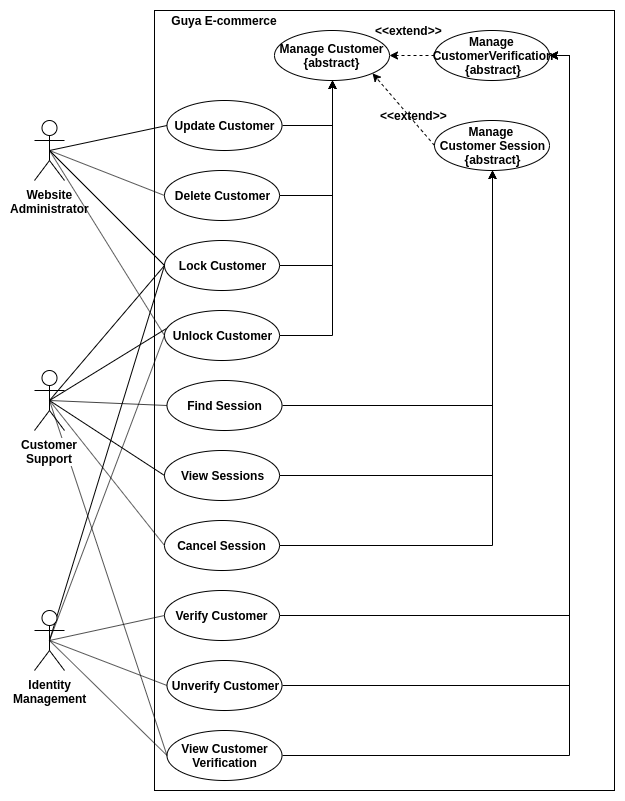
\includegraphics[width=10cm,keepaspectratio]{usecases/manage_customers_usecase}
\caption{Mange customer use case diagram for administration website - Guya E-commerce}
\end{figure}
%################################# End Of Manage customer #############################

%################################# Manage customer complaint #############################
\begin{figure}[!ht]
\centering
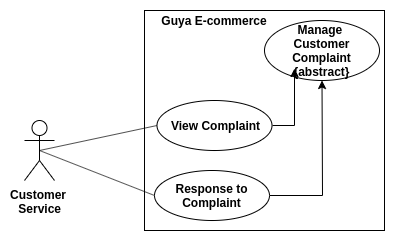
\includegraphics[width=10cm,keepaspectratio]{usecases/manage_customer_complaint}
\caption{Manage customer complaint use case diagram for administration website - Guya E-commerce}
\end{figure}
%################################# End Of Manage customer complaint #############################

\clearpage

%################################# Manage catalog #############################
\begin{figure}[!ht]
\centering
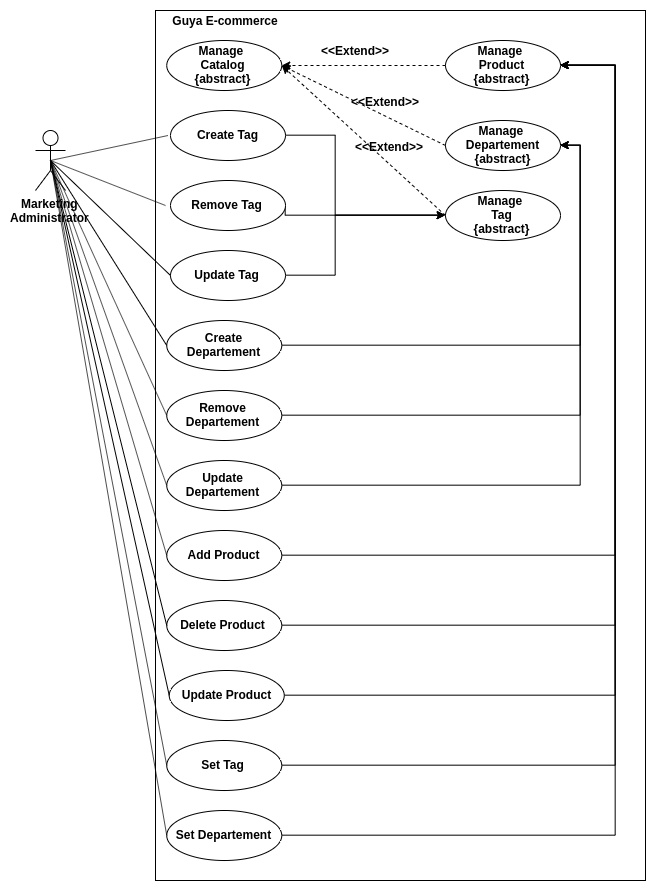
\includegraphics[width=15cm,keepaspectratio]{usecases/manage_catalog}
\caption{Mange catalog use case diagram for administration website - Guya E-commerce}
\end{figure}
%################################# End Of Manage catalog #############################

\clearpage

%################################# Manage promotion #############################
\begin{figure}[!ht]
\centering
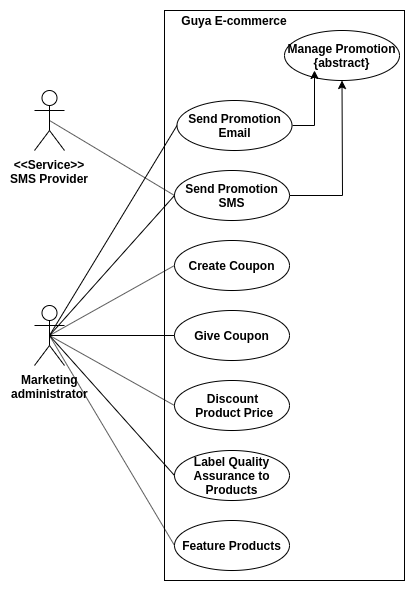
\includegraphics[width=10cm,keepaspectratio]{usecases/manage_promotion}
\caption{Manage promotion use case diagram for administration website - Guya E-commerce}
\end{figure}
%################################# End Of Manage promotion #############################

%################################# Manage inventory #############################
\begin{figure}[!ht]
\centering
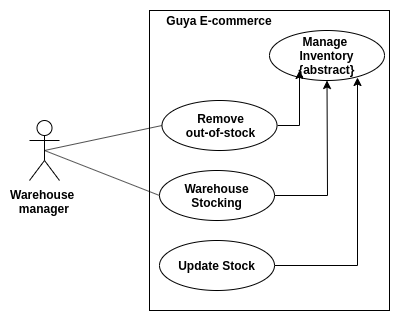
\includegraphics[width=10cm,keepaspectratio]{usecases/manage_inventory}
\caption{Manage inventory use case diagram for administration website - Guya E-commerce}
\end{figure}
%################################# End Of Manage inventory #############################

%################################# Manage delivery orders #############################
\begin{figure}[!ht]
\centering
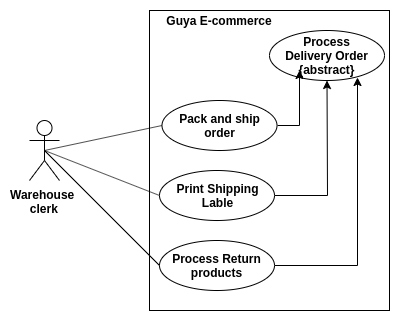
\includegraphics[width=10cm,keepaspectratio]{usecases/manage_delivery_order}
\caption{Manage delivery orders use case diagram for administration website - Guya E-commerce}
\end{figure}
%################################# End Of Manage delivery orders #############################
\clearpage
%################################# Manage branchs #############################
\begin{figure}[!ht]
\centering
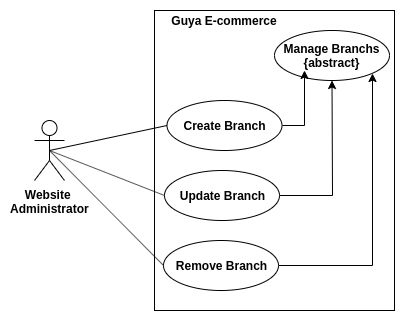
\includegraphics[width=10cm,keepaspectratio]{usecases/manage_branchs}
\caption{Manage branches use case diagram for administration website - Guya E-commerce}
\end{figure}
%################################# End Of Manage branchs #############################

\paragraph{Customer Use Case Diagram}
\clearpage
\begin{figure}
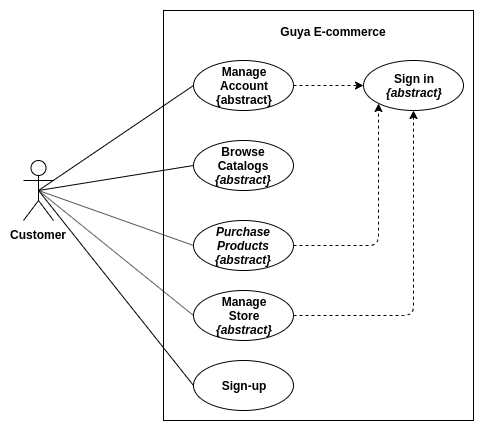
\includegraphics[width=15cm,keepaspectratio]{usecases/customer_top_level_usecase}
\caption{Top level use case diagram for the customer website - Guya E-commerce}
\end{figure}

%################################# Sign in  #############################
\begin{figure}[!ht]
\centering
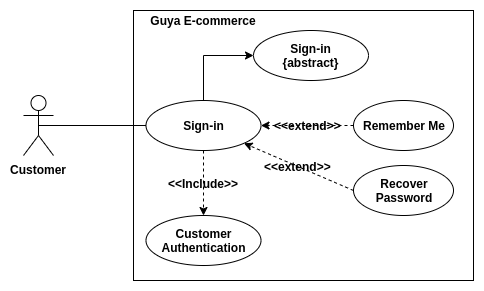
\includegraphics[width=10cm,keepaspectratio]{usecases/signin_usecase}
\caption{Sign in use case diagram for customer website - Guya E-commerce}
\end{figure}
%################################# End Of sign in #############################

%################################# Manage account #############################
\begin{figure}[!ht]
\centering
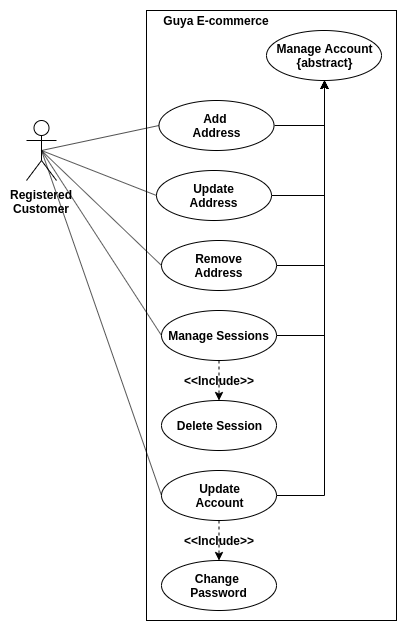
\includegraphics[width=10cm,keepaspectratio]{usecases/manage_account}
\caption{Manage account use case diagram for customer website - Guya E-commerce}
\end{figure}
%################################# End Of Manage account #############################

%################################# Brwose cataloge #############################
\begin{figure}[!ht]
\centering
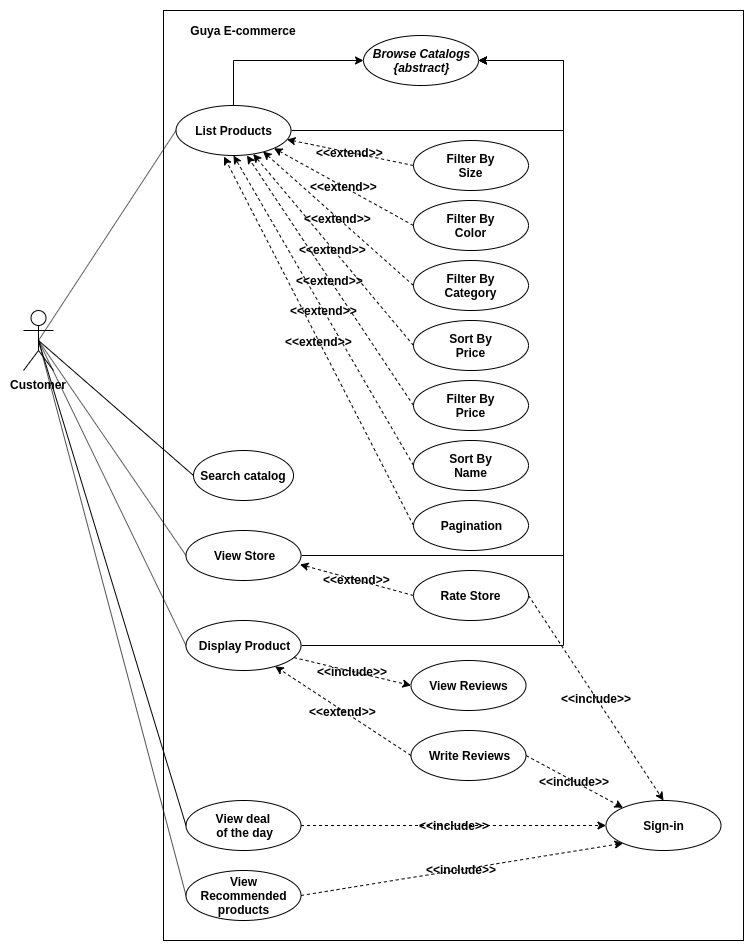
\includegraphics[width=15cm,keepaspectratio]{usecases/brwose_catalog}
\caption{Browse catalog use case diagram for customer website - Guya E-commerce}
\end{figure}
%################################# End Of Brwose cataloge #############################


\begin{figure}[!h]
%\vspace*{-2cm}
\hspace*{-3cm}
%\noindent
%\includegraphics[width=\paperwidth, height=\paperheight,keepaspectratio]{}  
\caption{Use case diagram overall system - Guya Express}
\end{figure}
\clearpage

%################################# Login #############################
\begin{table}[!ht]
\begin{tabular}{|l|p{6cm}|p{6cm}|}
\hline 
\rule[-1ex]{0pt}{2.5ex} \textbf{Use Case Name} & \multicolumn{2}{p{10cm}|}{Sign-in} \\ 
\hline 
\rule[-1ex]{0pt}{2.5ex} \textbf{Description} &\multicolumn{2}{p{10cm}|}{This Use Case describes the process by which users log into the order processing system. It also sets up access permissions for various categories of users} \\ 
\hline 
\rule[-1ex]{0pt}{2.5ex} \textbf{Primary Actor}& \multicolumn{2}{p{10cm}|}{Customer} \\ 
\hline 
\rule[-1ex]{0pt}{2.5ex} \textbf{Pre-Condition} & \multicolumn{2}{c|}{sign-up} \\ 
\hline 
\rule[-1ex]{0pt}{2.5ex} \textbf{Post-Condition} & \multicolumn{2}{p{10cm}|}{}  \\ 
\hline 
\multirow{8}{*}{\textbf{Basic Flow}} & \textbf{Actor Action} & \textbf{System Response}\\
%
&
\textbf{1.}  The Use Case starts when the user starts the application.
& 
\textbf{2.}  The system will display the login screen.
\\
%
&
\textbf{3.}  The user enters a username and password.
& 
\textbf{4.}  The system will verify the information. 
\\
%
&

& 
\textbf{5.}  The system will verify the information. 
\\
%
&

& 
\textbf{6.}  The system will set server session. 
\\
%
&

& 
\textbf{7.}  The system will set access permissions. 
\\
%
&
\textbf{8.}  The system will display the user's home screen.
& 
\textbf{9.}  The Use Case ends. 
\\
\hline 
\rule[-1ex]{0pt}{2.5ex} \textbf{Alternate Flow} & \multicolumn{2}{p{10cm}|}{If the credentials are wrong \& try's more than three times IP address will be captured and locked for sometime.}  \\ 
\hline 
\end{tabular}
\caption{Use Case Login - Guya E-commerce and Guya Express} 
\end{table}
%################################# End Of Login #############################


%################################# Login #############################
\begin{table}[!ht]
\begin{tabular}{|l|p{6cm}|p{6cm}|}
\hline 
\rule[-1ex]{0pt}{2.5ex} \textbf{Use Case Name} & \multicolumn{2}{p{10cm}|}{Register/Sign-up} \\ 
\hline 
\rule[-1ex]{0pt}{2.5ex} \textbf{Description} &\multicolumn{2}{p{10cm}|}{This Use Case describes the process by which users newly registering customer} \\ 
\hline 
\rule[-1ex]{0pt}{2.5ex} \textbf{Primary Actor}& \multicolumn{2}{p{10cm}|}{Customer} \\ 
\hline 
\rule[-1ex]{0pt}{2.5ex} \textbf{Pre-Condition} & \multicolumn{2}{c|}{} \\ 
\hline 
\rule[-1ex]{0pt}{2.5ex} \textbf{Post-Condition} & \multicolumn{2}{p{10cm}|}{}  \\ 
\hline 
\multirow{8}{*}{\textbf{Basic Flow}} & \textbf{Actor Action} & \textbf{System Response}\\
%
&
\textbf{1.}  The Use Case starts when the user opens the registering page.
& 
\textbf{2.}  The system will display the register screen.
\\
%
&
\textbf{3.}  The user fills the provided form.
& 
\textbf{4.}  The system will verify the information. 
\\
%
&

& 
\textbf{5.}  The system will either send E-mail verification link or cell phone number verification code, or both. 
\\
%
&
\textbf{6.}  The user will user will click on E-mail sent link or enter sent SMS code, or both. 
& 
\textbf{7.}  The user will user will verify user's email address or cell phone number, or both
\\
%
&

& 
\textbf{7.}  The system will log-in (sign-in) to the system. 
\\
%
&

& 
\textbf{9.}  The Use Case ends. 
\\
\hline 
\rule[-1ex]{0pt}{2.5ex} \textbf{Alternate Flow} & \multicolumn{2}{p{10cm}|}{If the verification link, SMS haven't reached the user the system will resend it.}  \\ 
\hline 
\end{tabular}
\caption{Register/Sign-up use case description - Guya E-commerce and Guya Express} 
\end{table}
%################################# End Of Login #############################

%################################# Employee Login #############################
\begin{table}[!h]
\begin{tabular}{|l|p{6cm}|p{6cm}|}
\hline 
\rule[-1ex]{0pt}{2.5ex} \textbf{Use Case Name} & \multicolumn{2}{p{10cm}|}{Staff Login} \\ 
\hline 
\rule[-1ex]{0pt}{2.5ex} \textbf{Description} &\multicolumn{2}{p{10cm}|}{This Use Case describes the process by which employee log into the order processing system. It also sets up access permissions for various categories of Employee types} \\ 
\hline 
\rule[-1ex]{0pt}{2.5ex} \textbf{Primary Actor}& \multicolumn{2}{p{10cm}|}{Customer} \\ 
\hline 
\rule[-1ex]{0pt}{2.5ex} \textbf{Pre-Condition} & \multicolumn{2}{c|}{sign-up} \\ 
\hline 
\rule[-1ex]{0pt}{2.5ex} \textbf{Post-Condition} & \multicolumn{2}{p{10cm}|}{}  \\ 
\hline 
\multirow{8}{*}{\textbf{Basic Flow}} & \textbf{Actor Action} & \textbf{System Response}\\
%
&
\textbf{1.}  The Use Case starts when the user starts the application.
& 
\textbf{2.}  The system will display the login screen.
\\
%
&
\textbf{3.}  The user enters a username and password.
& 
\textbf{4.}  The system will verify the information. 
\\
%
&

& 
\textbf{5.}  The system will verify the information. 
\\
%
&

& 
\textbf{6.}  The system will set access permissions. 
\\
%
&
\textbf{7.}  The system will display the user's home screen.
& 
\textbf{8.}  The Use Case ends. 
\\
\hline 
\rule[-1ex]{0pt}{2.5ex} \textbf{Alternate Flow} & \multicolumn{2}{p{10cm}|}{If the credentials are wrong \& try's more than three times IP address, staff credentials will be captured and locked for further analysis.}  \\ 
\hline 
\end{tabular}
\caption{Use Case Employee Login - Guya Express} 
\end{table}
%################################# End Of Employee Login #############################



\clearpage
\subsection{Activity Diagram}
Are graphical representations of workflows of stepwise activities and actions with support for choice, iteration and concurrency. In the Unified Modeling Language, activity diagrams are intended to model both computational and organizational processes (i.e., workflows), as well as the data flows intersecting with the related activities. Although activity diagrams primarily show the overall flow of control, they can also include elements showing the flow of data between activities through one or more data stores.\footcite{wikiactivitydiagram}

%\subsubsection{Action States and Activity States}
%\begin{itemize}
%	\item Action states are atomic and cannot be decomposed
%	\item Work of the action state is not interrupted.
%	\item Activity states can be further decomposed
%	\item Their activity being represented by other activity diagrams
%	\item They may be interrupted
%	\item Represented in UML by a rounded rectangle.
%	\item Activity represents the performance of some behavior in the work flow.
%\end{itemize}

%\begin{figure}[h]
%\center
%\begin{tikzpicture}
%\node (proc1) [process] {Activity/Process};
%\end{tikzpicture}
%\caption{Modified E-R Diagrams Description}
%\end{figure}

%\subsubsection{Transitions}
%Transitions are used to show the passing of the flow of control from activity to activity. They are %typically triggered by the completion of the behavior in the originating activity.
--%

Below figure describes activity diagram for both sub-projects any for any user i.e Administrative and Customer Login
\begin{figure}[!h]
\label{login_activity_diagram}
\center
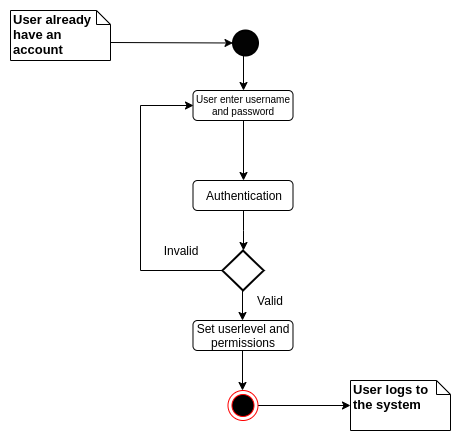
\includegraphics[width=10cm,keepaspectratio]{activity-diagrams/login_activity_diagram}
\caption{Login activity diagram - Guya E-commerce and Guya Express}
\end{figure}

\clearpage
\begin{figure}[!h]
\center
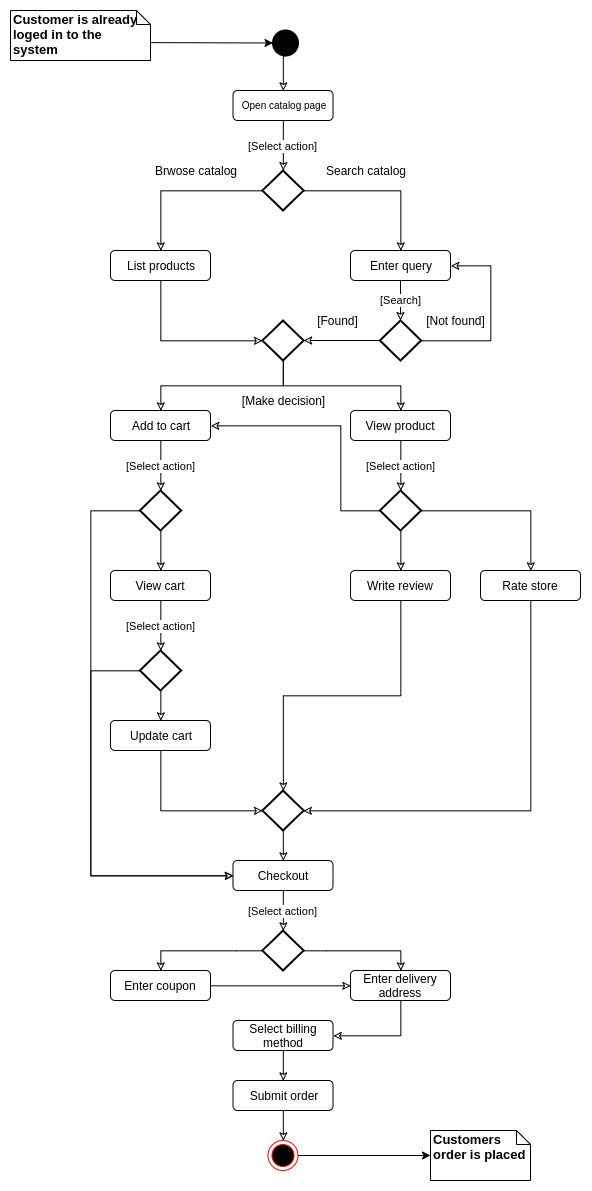
\includegraphics[width=12cm,keepaspectratio]{activity-diagrams/checkout_activity}
\caption{Check out activity diagram - Guya E-commerce}
\end{figure}

\clearpage
\begin{figure}[!h]
\hspace*{-3cm}
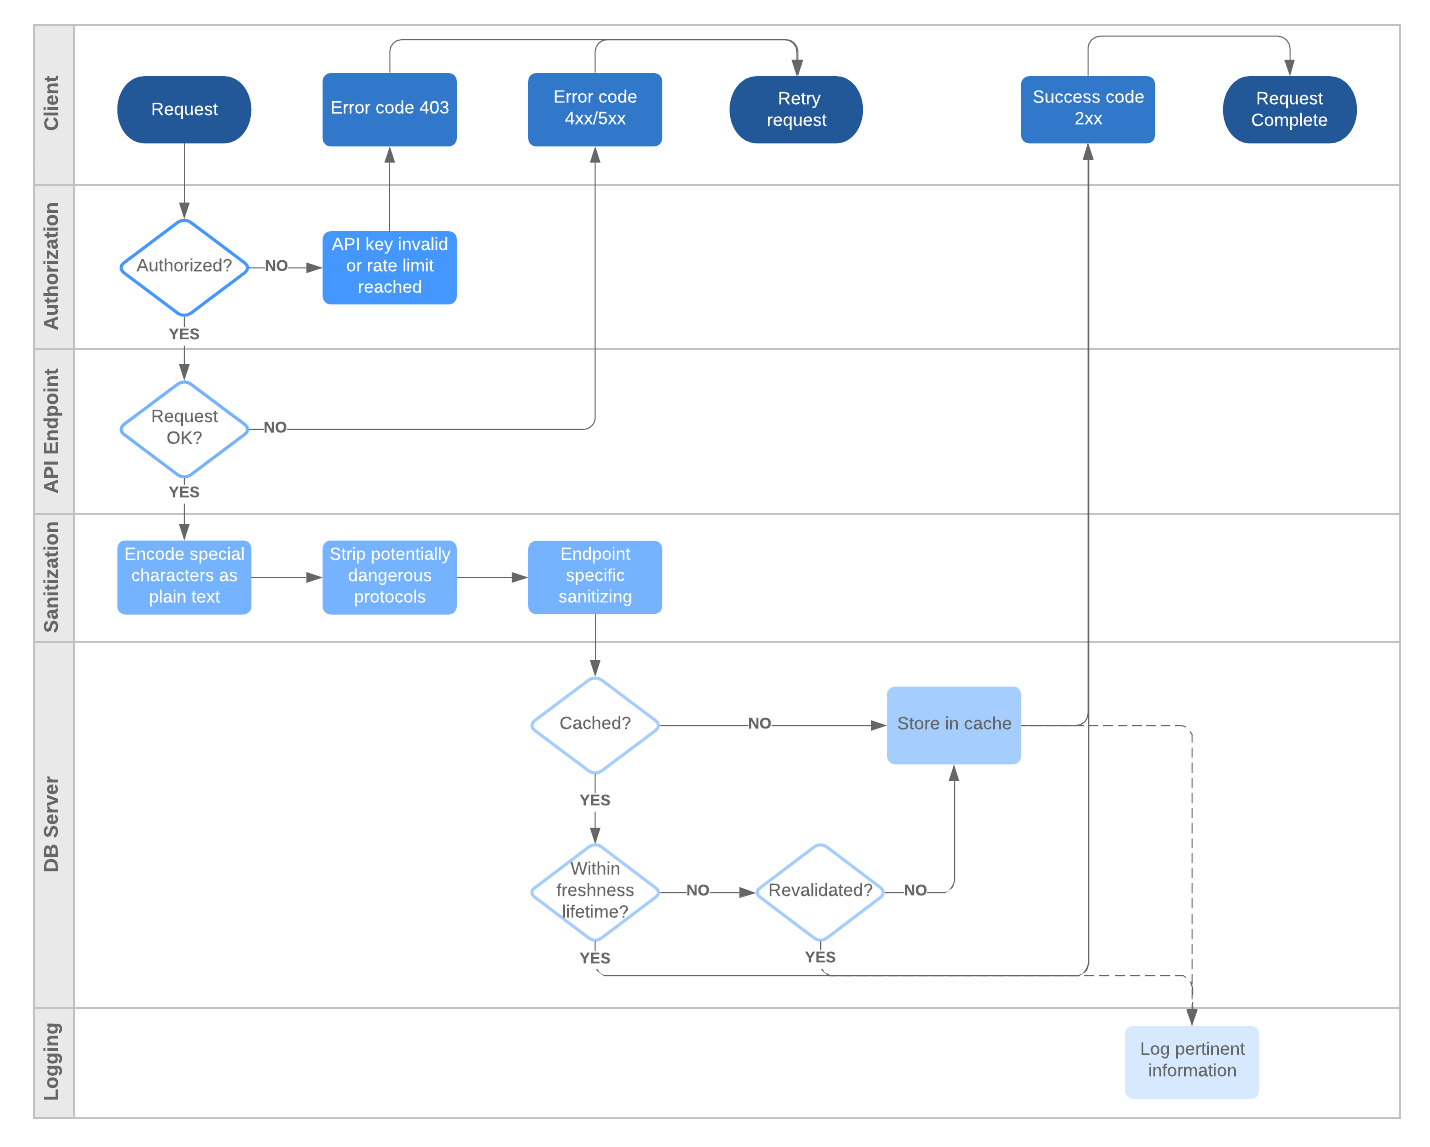
\includegraphics[width=\paperwidth, height=\paperheight,keepaspectratio]{activity-diagrams/api-flowchart-with-swimlanes}
\caption{Api Flowchart with swimlanes - Guya E-commerce and Guya Express }
\end{figure}
\clearpage



\subsection{Sequence Diagram}
\begin{figure}[!h]
\center
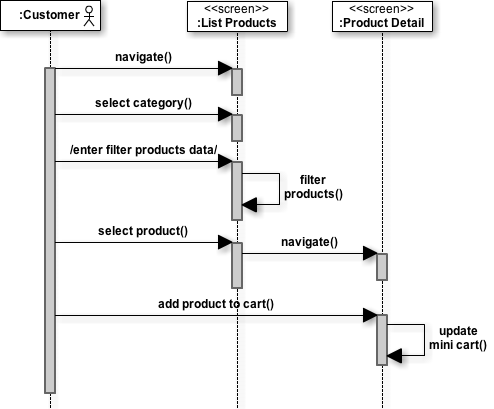
\includegraphics[keepaspectratio, width=15cm]{sequence-diagrams/catalog-storyboard.png}
\caption{Storyboard sequence of the browse catalog top-level use case - Guya E-commerce}
\end{figure}

\begin{figure}[!h]
\center
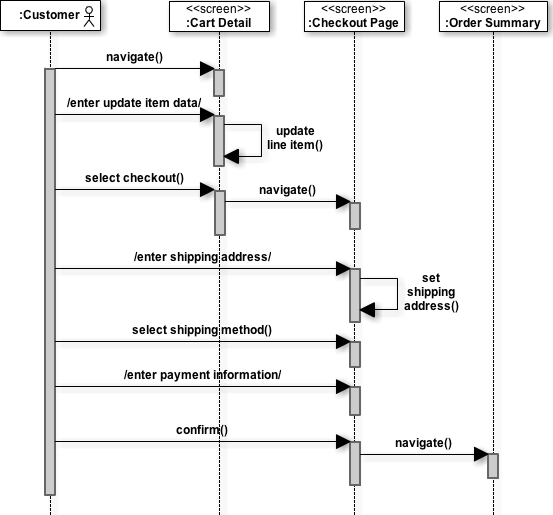
\includegraphics[keepaspectratio, width=15cm]{sequence-diagrams/checkout-storyboard.png}
\caption{Storyboard sequence of the checkout top-level use case - Guya E-commerce}
\end{figure}

\begin{figure}[!h]
\center
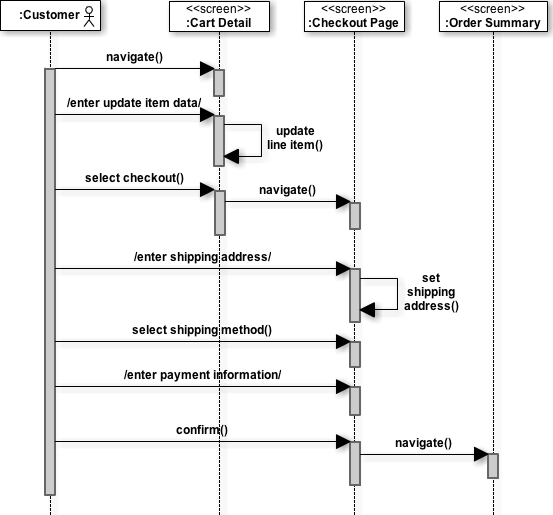
\includegraphics[keepaspectratio, width=15cm]{sequence-diagrams/checkout-storyboard.png}
\caption{Storyboard sequence of the check order top-level use case - Guya E-commerce}
\end{figure}

\begin{figure}[!h]
\center
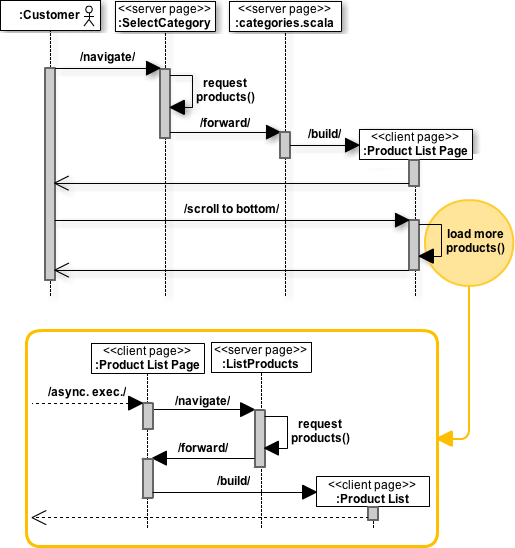
\includegraphics[keepaspectratio, width=15cm]{sequence-diagrams/pagination.png}
\caption{Internal design sequence diagram of the pagination - Guya E-commerce}
\end{figure}

\begin{figure}[!h]
\center
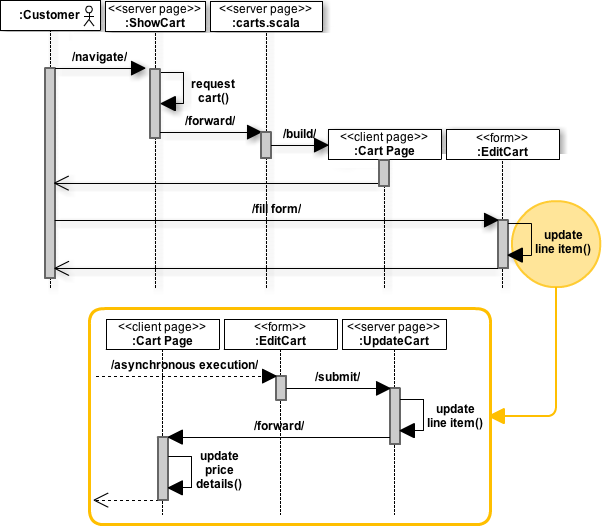
\includegraphics[keepaspectratio, width=15cm]{sequence-diagrams/update-cart.png}
\caption{Internal design sequence diagram of the update item in cart - Guya E-commerce}
\end{figure}

\begin{figure}[!h]
\center
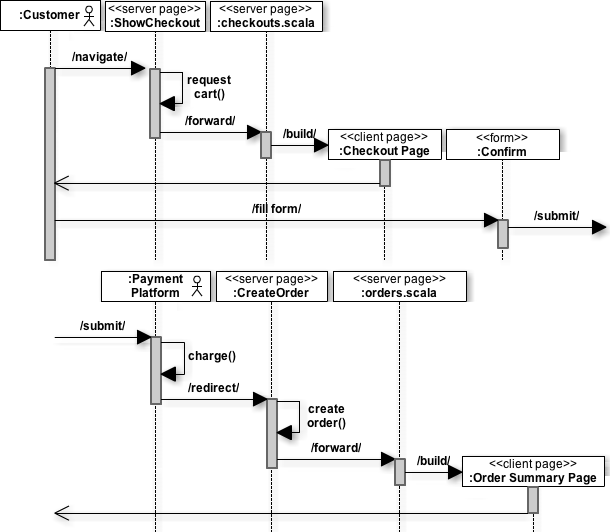
\includegraphics[keepaspectratio, width=15cm]{sequence-diagrams/order-and-payment.png}
\caption{Internal design sequence diagram of the place order and payment - Guya E-commerce}
\end{figure}

\begin{figure}[!h]
\center
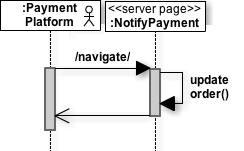
\includegraphics[keepaspectratio, width=7cm]{sequence-diagrams/payment-notification.png}
\caption{Internal design sequence diagram of the notification event in the payment - Guya E-commerce}
\end{figure}

\begin{figure}[!h]
\center
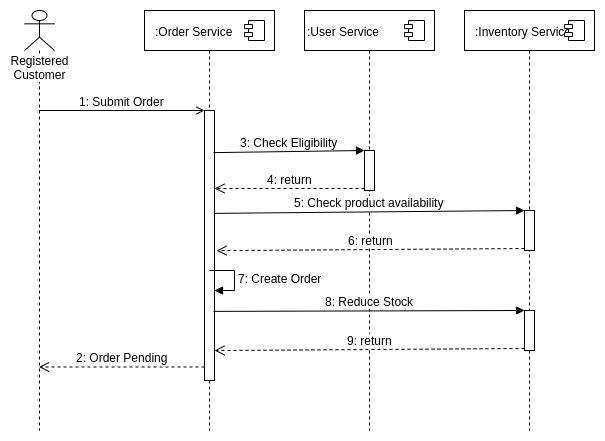
\includegraphics[width=15cm,keepaspectratio]{sequence-diagrams/order_sequence}
\caption{Ordering sequence diagram - Guya E-commerce}
\end{figure}

\begin{figure}[!h]
\center
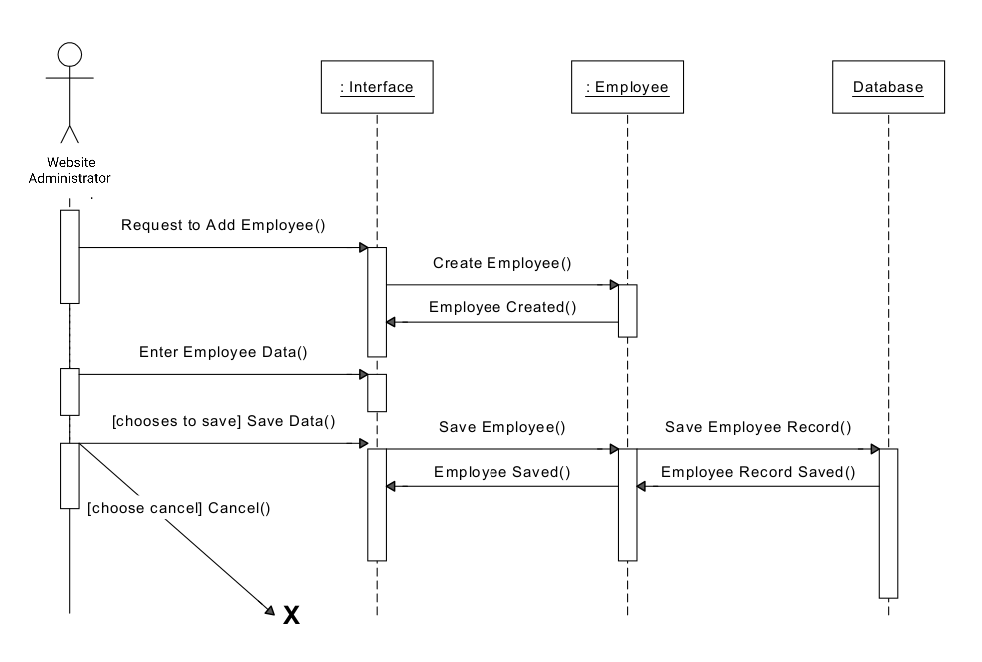
\includegraphics[width=15cm,keepaspectratio]{sequence-diagrams/employee_sequence}
\caption{Add employee/staff sequence diagram - Guya Express}
\end{figure}

\begin{figure}[!h]
\center
\includegraphics[width=15cm,keepaspectratio]{sequence-diagrams/jwtt_sequnce}
\caption{JWT security authentication - Guya E-commerce and Guya Express}
\end{figure}

\clearpage
  
\subsection{State Diagrams}
There are two interesting state diagrams of this system, both related to the cart element. The first diagram (Figure \ref{cart-state-diagram}) describes how a cart instance changes until it becomes a complete order. As the diagram below shows, the current cart is the initial state, which allows to change its contents in multiple ways, such as adding or removing line items or selecting a shipping address. Once the checkout is finished the cart becomes an order, being this an irreversible change. From now on the order can only change from an open to a complete state, and vice versa.

\begin{figure}[!h]
\center
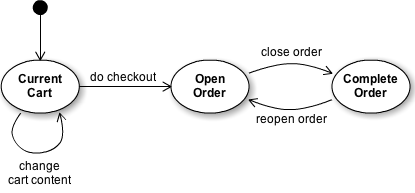
\includegraphics[keepaspectratio, width=10cm]{state-diagrams/cart-state-diagram.png}
\caption{State diagram of the cart class - Guya E-commerce}
\label{cart-state-diagram}
\end{figure}

The second diagram (Figure 3.12) describes the whole process of managing the shopping cart and eventually purchasing these products in the checkout process. This diagram will become especially useful when designing the checkout interface, as it clearly displays the requirements of each step of the checkout process.

\begin{figure}[!h]
\center
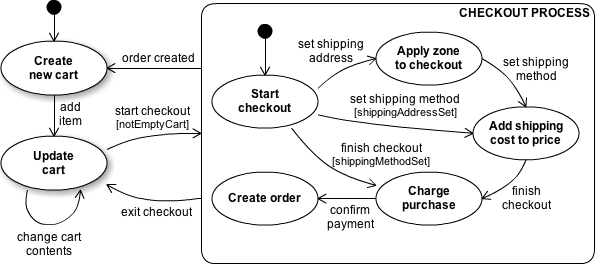
\includegraphics[keepaspectratio, width=15cm]{state-diagrams/purchasing-product-state-diagram.png}
\caption{State diagram of the cart class - Guya E-commerce}
\label{purchasing-product-state-diagram}
\end{figure}

At the beginning of the process a new cart is created. Once the cart contains an item it can be further updated, then at any moment the user can start or exit the checkout process. Initially the checkout process requires a shipping address to display the shipping methods, then it requires a shipping method to display billing options. Of course this sequence can be skipped if the cart has already these requirements.
When the user provides the billing information and finalizes the checkout, the system charges the customer. The order is then created after the payment platform confirms that the payment was successful. The moment the previous cart becomes an order, a new cart is created for the customer in order to start the process once again.


\subsection{Analysis Class Diagram}
In the world of information architecture, UML still has a strong foothold. Therefore class diagrams are still desired, even when designing RESTful APIs, We have there sought a way to represent that pieces that make up an 	API as UML and found that although this is somewhat intuitive, there is not one set way of doing this.

Identifying variable (properties) which is done by writing $<<$representation$>>$ below it is the representation name, identifying resources is done by writing $<<$resource$>>$ below the resource is the name of REST API name. In the methods variables, variable that begins with a capital letter represent a set(array or json) of messages, except for Accept-Language which is a header, which are refereed to (mapped to) representation and for the arrow is a path. For example for login resource the resource name is login, representation/message is Login, path is /v1/users/login and method will be put(Accept-Language, [username, password]). See Chapter 3 Class Diagram Description


%\begin{figure}[!h]
%\vspace*{-8cm}
%\hspace*{-3cm}
%\noindent
%\includegraphics[height=22cm, angle=90, keepaspectratio]{}
%\caption{Class diagram (API diagram) - Guya E-commerce}
%\end{figure}
%\clearpage


